\section{Introduction}
Network monitoring is a major building block for many domains in communication networks.
Besides typical accounting mechanisms and the emerging area of charging in next generation networks, especially network security solutions rely on efficient means of monitoring.

In order to cope with the increasing amounts of monitoring data brought about by ever-growing network capacities, monitoring is commonly based on flow accounting and statistical packet sampling. 
In accordance with the terminology used in the literature, we use the term \emph{flow} to designate a stream of packets sharing a set of common properties (called flow keys) like end point addresses or used protocol.
Usually, a flow is defined by the IP-quintuple \texttt{<proto, src\_ip, dst\_ip, src\_port, dst\_port>}, but arbitrarily chosen flow keys are also allowed -- even keys that depend on user-defined field types.

The techniques for flow accounting, as well as the transfer of observed monitoring data, are set out in the Cisco NetFlow.v9 protocol~\cite{rfc3954} and its successor, the IPFIX (IP Flow Information Export) protocol~\cite{ietf-ipfix-protocol}.
In contrast to IPFIX, that carries flow information, the PSAMP (Packet Sampling) protocol~\cite{ietf-psamp-protocol} was developed to satisfy the growing need for more detailed network monitoring.
PSAMP gathers samples of individual packets and allows exporting of actual payload.
Both the IPFIX protocol and the PSAMP protocol are being standardized by the IETF (Internet Engineering Task Force).
Figure~\ref{fig_ipfix_arch} illustrates the functional architecture of an IPFIX/PSAMP device consisting of Metering Processes (MP), Sampling Processes (SP), Aggregation Processes (AP), Collecting Processes (CP), and Exporting Processes (EP), that can be linked in various ways.

\begin{figure}
\begin{center}
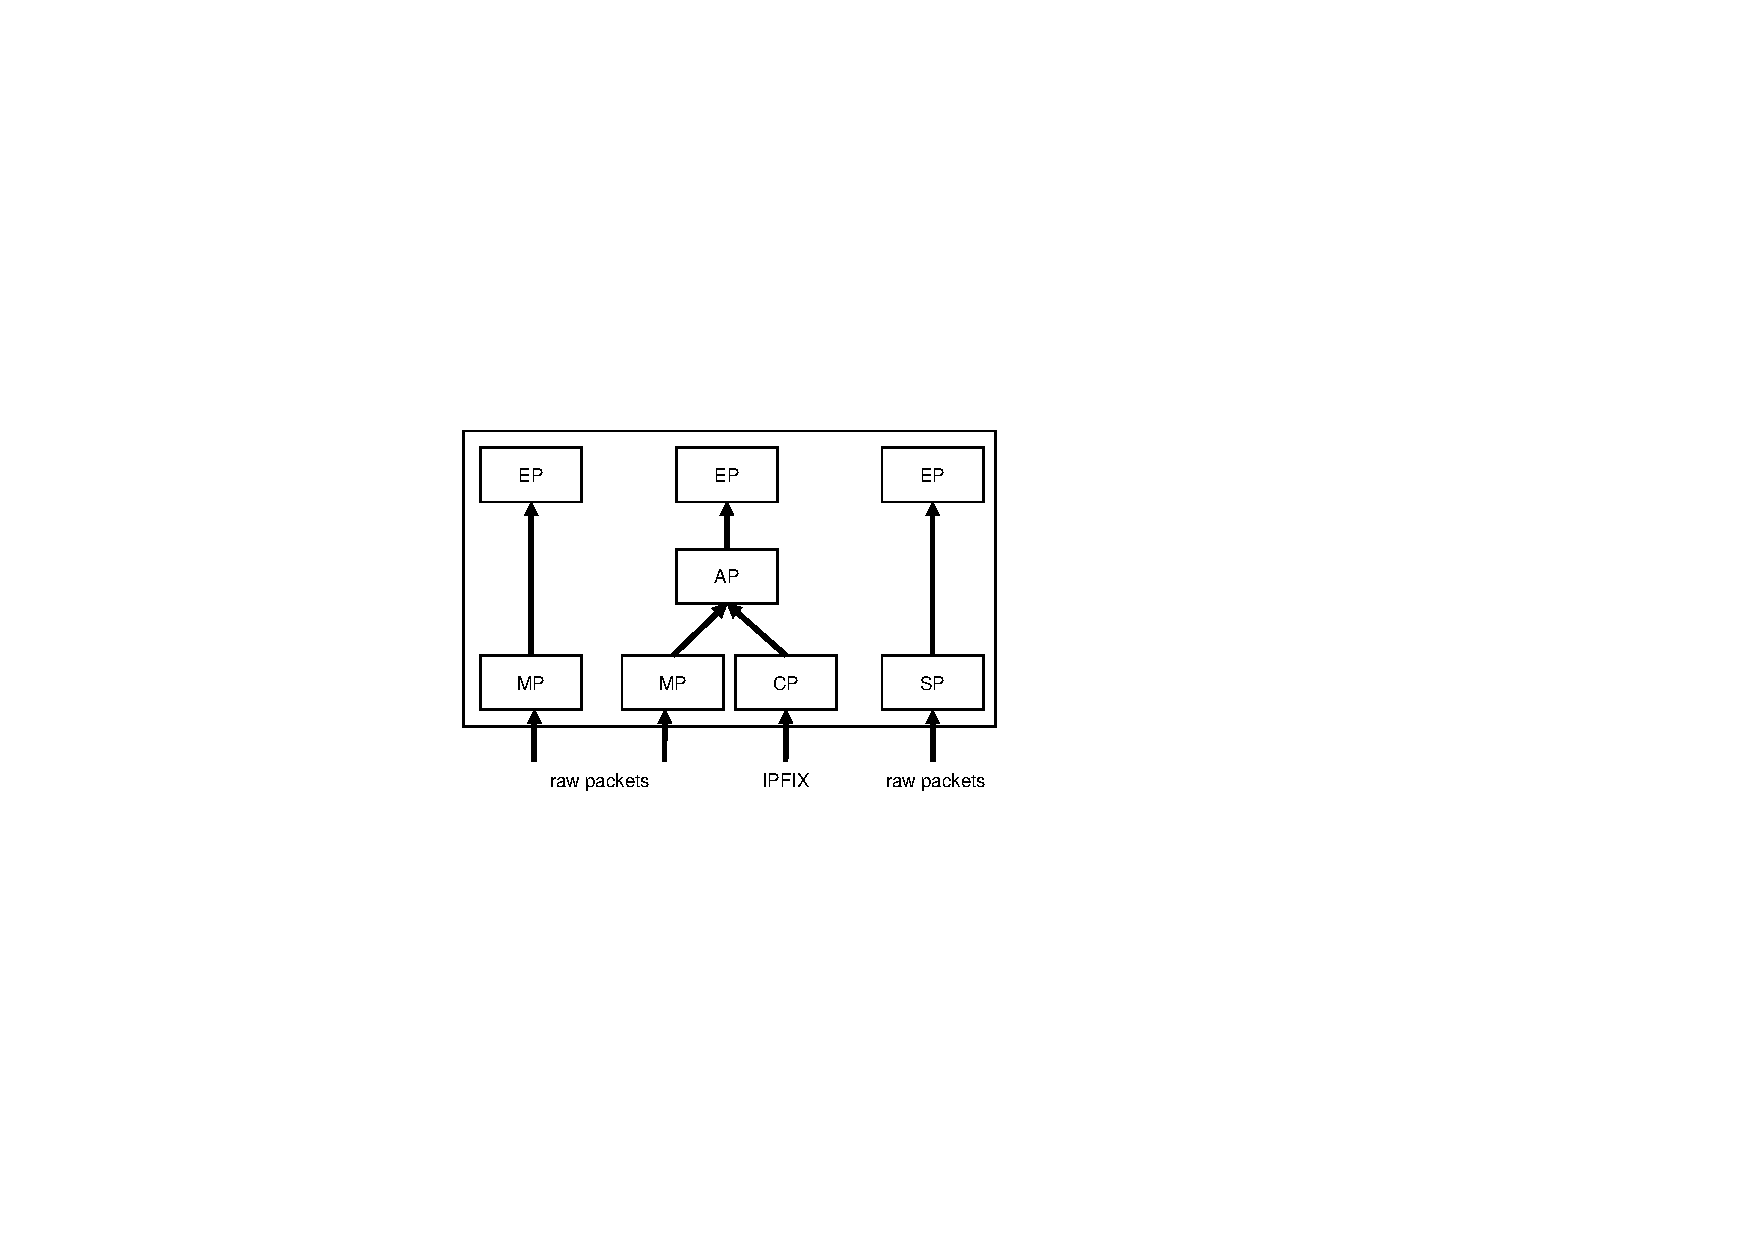
\includegraphics[scale=0.55]{gfx/ipfix-arch2.pdf}
\caption{IPFIX Device Architecture: Metering, collecting and sampling processes feed data to aggregation and exporting processes}
\label{fig_ipfix_arch}
\end{center}
\end{figure}


In this paper, we present the monitoring toolkit Vermont, which has been developed in the \emph{History} project~\cite{dressler2005history} and the European project \emph{Diadem Firewall}.
Vermont was designed for monitoring high-speed networks with link speeds of up to one gigabit per second using standard PC hardware.
Furthermore, Vermont serves as a reference implementation of the aforementioned monitoring techniques, including the protocol extensions for flow aggregation~\cite{dressler-ipfix-aggregation}.

The design principles of Vermont are:
\begin{itemize}
\item IPFIX/PSAMP conformant monitoring and data export
\item Rule-based flow metering and aggregation
\item Hardware-independent packet capturing
%\item Efficient, decoupled data processing
\item Multiprocessor support
\item High monitoring performance
\end{itemize}

The remainder of this paper is organized as follows.
Section~\ref{sec:related-work} briefly introduces other open-source implementations of monitoring probes and compares them to Vermont.
Section~\ref{sec:architecture} outlines Vermont's architecture.
Application scenarios are provided in section~\ref{sec:scenarios} and results obtained in performance, compatibility, and robustness evaluations are discussed in section~\ref{sec:evaluation}.
Finally, section~\ref{sec:conclusion} concludes the paper.

